% !TeX root = ../tesis.tex

\chapter*{Background and Motivation}
\addcontentsline{toc}{chapter}{\protect\numberline{}Background and Motivation}	  		% Comment if you don't want the introduction to appear on the table of content. It will not have a number
\label{chapter:intro}

% this file is called up by thesis.tex
% content in this file will be fed into the main document


Optical metasurfaces are bidimensional arrays of metallic/dielectric nanostructures ---known as meta-atoms--- specifically tailored to behave in a way no found in nature when illuminated at a specific wavelength \cite{khan_optical_2022,gonzalez-alcalde_large_2020}. Depending on the physical properties of the meta-atoms, that is, their material, size, shape, and orientation and distribution within the bidimensional array \cite{kim_plasmonic_2019,khan_optical_2022}, metasurfaces allow to shape at will the  spatial optical response of the system \cite{chen_review_2016}, thus suiting them for a variety of applications in fields such as spectroscopy \cite{khan_optical_2022}, color structuration \cite{gonzalez-alcalde_large_2020}, communications \cite{chen_review_2016}, and sensing \cite{estevez_trends_2014,jain_noble_2008,khan_optical_2022,chen_review_2016,kim_plasmonic_2019}. In the last decades, the interest in optical metasurfaces for medical applications has increased due to  the need for sensitive, fast, low-cost and easy-to-use technologies \cite{estevez_trends_2014,kim_plasmonic_2019}, like metasurfaces with plasmonic (metallic) meta-atoms used as contrasting agents for bioimaging  \cite{kim_plasmonic_2019}, and as free-label biosensors returning real-time measurements \cite{estevez_trends_2014,kabashin_plasmonic_2009,khan_optical_2022}.

Metasurfaces designed for biosensing typically consist of a nanostructurated substrate with compatible microfluidics illuminated with a white light source and a light recollection system, allowing for scattering or extinction measurements, followed by an spectrometer \cite{estevez_trends_2014,feuz_improving_2010}. One particular kind of  biosensing-aimed metasurfaces consists in plasmonic meta-atoms, exploiting their property of high confinement of light at nanometric scales, yielding an improvement in the sensitivity of various detection techniques \cite{khan_optical_2022}. The light confinement is the result of the meta-atom's Localized Surface Plasmon Resonances (LSPRs) being excited at the meta-atom's interface with its surroundings, which occurs when the electromagnetic fields couple to the free electrons of the plasmonic structure \cite{chen_review_2016,kim_plasmonic_2019,estevez_trends_2014}.  Since the LSPR is material and geometry dependent, a variety of plasmonic metasurfaces have been designed \cite{feuz_improving_2010,kabashin_plasmonic_2009,qiu_dual_2020,svedendahl_refractometric_2014} ---each with its own benefits and disadvantages \cite{chen_review_2016,estevez_trends_2014}--- as those shown in  Fig. \ref{fig:Back}, all of which are plasmonic metasurfaces consisting of gold (Au) meta-atoms on a glass substrate but with different geometries and distributions within the metasurface.  For example, Feuz et al. \cite{feuz_improving_2010} employed a short-range ordered metasurface of nanoholes to sense protein binding events in real-time [Fig. \ref{sfig:back:a}], while  Kabashin et al. \cite{kabashin_plasmonic_2009} measured  changes in the refractive index of the media embedding an ordered metasurface of plasmonic nanorods [Fig. \ref{sfig:back:b}].  Metasurfaces with simpler geometries and distributions can be used  for biosensing as well, as shown Qiu et al. \cite{qiu_dual_2020}, who employed a disordered metasurface of nanospheres to detect selected DNA sequences from Severe Acute Respiratory Syndrome Coronavirus 2 (SARS-CoV-2) [Fig. \ref{sfig:back:c}], or by Svedendahl et al. \cite{svedendahl_refractometric_2014}, who sensed protein binding events with a short-range ordered metasurface of nanospheres [Fig. \ref{sfig:back:d}].

\begin{figure}[h!]
\centering
\hspace*{-3.5em}%
\begin{tikzpicture}[scale = .9]
	  \node at (0,0) {  \includegraphics[width = \textwidth]{background.png}};
		\node at (-8.3,4.15) {  \begin{subfigure}{.2\textwidth}\caption{ }\label{sfig:back:a}\end{subfigure}};
		\node at (-2.3,4.15) {  \begin{subfigure}{.2\textwidth}\caption{ }\label{sfig:back:b}\end{subfigure}};
		\node at (-2.3,-1) {  \begin{subfigure}{.2\textwidth}\caption{ }\label{sfig:back:c}\end{subfigure}};
		\node at (5.2,4.15) {  \begin{subfigure}{.2\textwidth}\caption{ }\label{sfig:back:d}\end{subfigure}};
\end{tikzpicture}
  \vspace*{-1.75em}
  \caption[Backgrounds]{Examples of biosensing-aimed plasmonic metasurfaces. \textbf{a)} Short-range ordered metasurface of nanoholes in a Au film [Scanning Electron Microscopy (SEM) image and meta-atom scheme] and real-time measurements of the LSPR redshift due to protein binding events; images extracted and adapted from \cite{feuz_improving_2010}. \textbf{b) } Reflectivity minimum shift of an ordered metasurface of Au nanorods (SEM image and scheme in the inset) as a function of the refractive index change of the media embedding the metasurface; images extracted and adapted from \cite{kabashin_plasmonic_2009}. \textbf{c)} Schematics of a disordered metasurface of Au nanospheres designed for SARS-CoV-2 detection and the LSPR response of its meta-atom: Thermoplasmonic and plasmonic sensing; image extracted from \cite{qiu_dual_2020}. \textbf{d)} Experimental and theoretical results for the ellipsometric parameter $\Delta$ as a function of the incident wavelength, when a short-ranged ordered metasurface of Au nanospheres (SEM image) is illuminated by a  non-polarized white light as shown in the setup diagram; extracted and adapted from \cite{svedendahl_refractometric_2014}.
  }
\label{fig:Back}
\end{figure}

The design of plasmonic metasurfaces undergo several stages, but it can be roughly divided in two: its fabrication process and its theoretical behavior. On the one hand, the fabrication process relies on a variety of methods depending on the desired meta-atom's physical properties and distribution. For example, metasurfaces suited for biosensing are commonly  fabricated by lithography techniques, like electron beam lithography (ordered array) or hole-mask colloidal lithography  (ordered and disordered arrays) \cite{estevez_trends_2014}, thermal annealing of thin metallic films (disordered arrays) by dewet \cite{qiu_dual_2020} or laser ablation \cite{meng_anisotropic_2015}, and chemical growth-methods \cite{estevez_trends_2014,kabashin_plasmonic_2009}. On the other hand, the theoretical behavior estimates the optical response of the metasurface either by numerical methods, like the Finite Element Method (FEM) \cite{feuz_improving_2010}, the Finite Differences Time Domain (FDTD) \cite{qiu_differential_2015}, and the Discrete Dipole Approximation (DDA) \cite{meng_anisotropic_2015}, or by analytical models, like the Thin Island Theory \cite{svedendahl_refractometric_2014,bedeaux_optical_2004}, the Dipolar Model \cite{barrera1991optical} ---both developed for disordered bidimensional arrays of nanospheres on a substrate--- or the Maxwell Garnett Model ---originally developed for 3D colloidal systems of spheres \cite{sihvola_electromagnetic_2008}--- modified to describe bidimensional systems of non-spherical meta-atoms \cite{oates_characterization_2011,kabashin_plasmonic_2009,moirangthem_enhanced_2012}. It is stressed that such calculations returns the optical response of the metasurface under ideal conditions as, for example, perfect geometrical shapes of the meta-atoms, perfect periodicity or even perfect deposition on the substrate supporting the meta-atoms.

Biosensing-aimed metasurfaces are supported on a substrate and immersed in an aqueous superstate \cite{estevez_trends_2014}, and its theoretical behavior is usually analyzed under the assumption that the meta-atoms are perfectly supported on the substrate and perfectly embedded in the superstate  \cite{kabashin_plasmonic_2009,qiu_differential_2015,barrera1991optical,svedendahl_refractometric_2014,bedeaux_optical_2004}. Nevertheless, a partial embedding of the meta-atoms into the substrate may arise experimentally depending on the parameters of the fabrication process  \cite{meng_anisotropic_2015,moirangthem_enhanced_2012}. The partial embedding of the meta-atoms is inversely related to the sensing area of the metasurface in the superstrate, thus limiting its performance, but it is also directly related to the washability of its meta-atoms due to the coupled microfluidics. Therefore, the partial embedding of the meta-atoms is a physical feature that can be optimized to design a long-lasting and sensitive metasurface for biosensing, yet, few publications on partially embedded nanostractures can be found even for simple geometries. Two examples of studies on partially embedded nanospheres are the results of Meng et al. \cite{meng_anisotropic_2015} and of Moirangthem et al. \cite{moirangthem_enhanced_2012}, who respectively compared the experimental optical response of disordered bidimensional arrays of Au nanospheres with different incrustation degrees [see for example Fig. \ref{sfig:inc:a}] employing DDA calculations of a single Au nanospheroid partially embedded and illuminated at normal incidence [Fig. \ref{sfig:inc:b}], and by substituting the partial embedded Au nanospheres by two thin films described optically with the Maxwell Garnett Model with fitting parameters [Fig. \ref{sfig:inc:c}] and a FDTD analysis for the spatial distribution of the electric near-field (not shown). While both publications mentioned before studied partially embedded meta-atoms (Au nanospheroids) neither of them focuses on their overall optical response,  on its comparison with perfectly deposited meta-atoms nor on the effects the partial embedding may have on a metasurfaces for biosensing.

\begin{figure}[h!]
\centering
\hspace*{-3.75em}%
\begin{tikzpicture}[scale = 1]
	  \node at (0,0) {  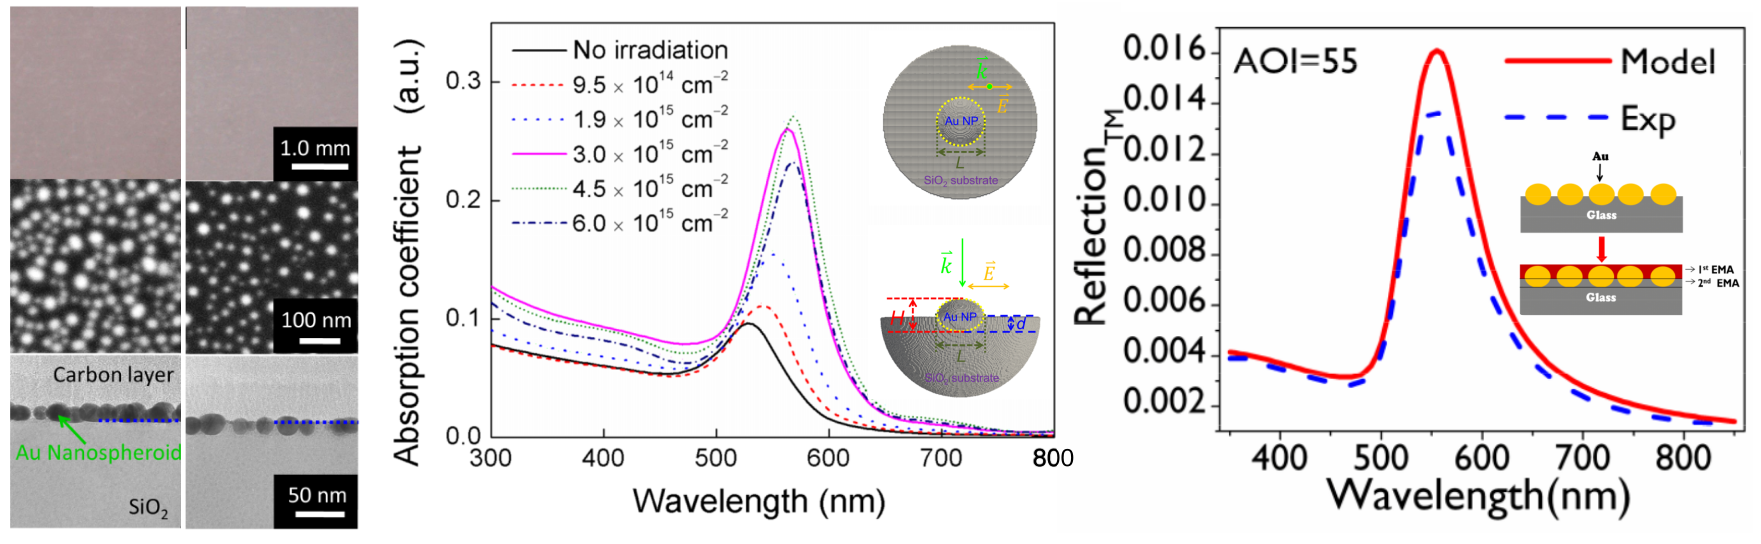
\includegraphics[width = .9\textwidth]{embedding.png}};
		\node at (-7.5,2.15) {  \begin{subfigure}{.2\textwidth}\caption{ }\label{sfig:inc:a}\end{subfigure}};
		\node at (-3.5,2.15) {  \begin{subfigure}{.2\textwidth}\caption{ }\label{sfig:inc:b}\end{subfigure}};
		\node at (1.725,2.15) {  \begin{subfigure}{.2\textwidth}\caption{ }\label{sfig:inc:c}\end{subfigure}};
\end{tikzpicture}
  \vspace*{-.75em}
  \caption[Backgrounds]{Previous works on partially embedded Au nanospheroids. \textbf{a)} Optical image and Transmission Electron Microscopy (TEM) images in an aerial and transversal view of disordered bidimensional arrays of nanospheres supported on silica  (SiO$_2$),  with two different incrustation degrees, fabricated by laser ablation of a Au thin film; image extracted and adapted from \cite{meng_anisotropic_2015}. \textbf{b) }  Absorption coefficient of a single Au nanospheroid ---with a depolarization factor $L$--- when illuminated at normal incidence by a plane wave, calculated with DDA (see inset) considering the measured dimensions and incrustration degree of the Au nanospheres; images extracted and adapted from \cite{meng_anisotropic_2015}.  \textbf{c)} Experimental and theoretical reflectivity, as a function of the wavelength, of a disordered bidimensional array of partially embedded Au nanospheres illuminated at an angle of incidence of $55^\circ$ with a transverse magnetic (TM) polarization state; the employed model consisted on substituting the partially embedded Au nanospheres by two layers whose optical response is described by the Maxwell Garnet Model with fitting parameters; images extracted and adapted from \cite{moirangthem_enhanced_2012}.
   }
\label{fig:IncPapers}
\end{figure}

In this thesis, the optical properties of a single Au nanosphere partially embedded in a substrate ---a potential meta-atom for biosensing-aimed metasurfaces---  are studied when illuminated by a monochromatic plane wave at an oblique incidence with a defined polarization state. The system of interests consists in a spherical Au nanoparticle of radius $12.5$ nm located at the planar interface between an air matrix and a glass substrate, whose embedding (including the perfectly supported and totally incrusted nanosphere) is characterized by the incrustation parameter: the height of the center of the nanosphere relative to the interface divided by its radius. To determine the optical response of the system, the scattering and absorption efficiencies, the radiation pattern and the spatial distribution of induced electric field of the partially embedded nanosphere are calculated by means of the FEM ---implemented in the commercial software COMSOL Multiphysics\texttrademark{} Ver. 5.4 (COMSOL)--- and they are compared with the results obtained with the Mie Theory ---the analytical solution of the limiting case of a single nanosphere embedded in a infinite medium---, which allows to estimate the performance of partially embedded nanoshperes in metasurfaces tailored for biosensing.

The structure of this thesis divides its contents in three main chapters as follows: the scatering theory of single spherical particles is presented in Chapter \ref{ch:OpticalProperties}, beginning with the general case of arbitrary particles in Section \ref{s:AmpMatCrossSect} and followed by the particular case of spherical scatterers,  giving rise to the development of the Mie Theory in Section \ref{s:Mie}, which includes the derivation of the Vector Spherical Harmonics (Section \ref{ss:VSH}) and the explicit solution to the scattered and internal electromagnetic fields (Section \ref{ss:Fields}); in Section \ref{ss:AuMie} the optical properties of a Au nanosphere of radius $12.5$ nm embedded in air, and in glass, are calculated as the Mie-limiting case to the system of interest. Chapter \ref{chapter:FEM} aims at providing the fundamentals of the FEM in Section \ref{s:FEM-Fund}, including the Galerkin Method in Section \ref{s:FEM-Fund} and the characteristics of the Finite Element Approximation to a problem of partial differential equations in Section \ref{ss:FEM-FE}, and how the light scattering problem is addressed in the FEM in Section \ref{s:Scat-FEM}, which yields its Strong and Weak formulations (Section \ref{ss:Scat-Form}), the kind of finite element suited for the light scattering problem ---the Nédélec Finite Element--- (Section  \ref{ss:Nedelec}), and the so-called Open Boundary Conditions (Section  \ref{ss:Sommerfeld-PML}) that allows to calculate optical properties for infinite non-periodic  systems, as that of a single partially embedded nanosphere; after the theory of the FEM is presented, a convergence analysis is presented in Section \ref{sec:FEM-Mie} for the FEM implementation in COMSOL where its results are compared against the analytical solutions calculated by the Mie Theory. Then, the obtained results and their discussion are presented in Chapter \ref{ch:Results}, which corresponds to the scattering and absorption efficiencies, the radiation patterns and the spatial distribution of the induced electric field of a Au nanosphere of radius $12.5$ nm under the following conditions: perfect support and total embedding in the substrate in Section \ref{s:Totally}, and partial embedding in Section \ref{s:Emb}; the first considers normal incidence illumination in both an internal and external illumination schema in Section \ref{s:Totally:Normal} and in a Total Internal Reflection Configuration (TIR) in Section \ref{s:TIR}, while the second addresses the normal illumination case only in internal illumination and the TIR configuration in Sections \ref{s:Emb:Normal} and \ref{s:Emb:Obl}, respectively. Lastly, the \hyperref[ch:Conclusions]{Conclusions} of this work and its \hyperref[s:FWork]{future application on Metasurfaces} are located after the three main chapters.	


As a complementary material, there are included three appendices describing the conventions employed for the calculations with the Mie Theory (Appendix \ref{app:MieCode}), the size correction to the dielectric function for small spherical nanoparticles (Appendix \ref{app:SizeCorrection}) ---both available in the public GitHub repository \href{https://github.com/jaurrutia/Mie-Theory-Mathematica}{jaurrutia/Mie-Theory-Mathematica}--- and a brief guide of how the performed calculations were implemented in COMSOL (Appendix \ref{app:COMSOL}).





